\subsection{Maximised Airspace Utilisation}

% To accommodate growing air traffic demand and integrate \gls{UAM}, airspace utilisation must be maximised efficiently and safely. 
% Two key EU-funded projects: Metropolis and Metropolis 2, have explored how structured airspace and separation management strategies can address these challenges.

The increasing demand for \gls{UAM} and the integration of \glspl{UAV} into controlled airspace present major challenges for traditional \gls{ATM}. 
To maximise the use of limited urban airspace while maintaining safety and efficiency, novel airspace design concepts and AI-driven separation management techniques are being explored.

% \subsubsection{Metropolis Project: Structuring the Airspace}

The first Metropolis project investigated how different airspace structures affect capacity, complexity, safety, and efficiency in high-density urban environments. 
It introduced four airspace concepts: Full Mix, Layers, Zones, and Tubes, each offering varying levels of structure to manage \gls{UAV} traffic (Figure~\ref{airspace-concepts}):

\begin{itemize}
    \item \textbf{Full Mix:} An unstructured airspace where aircraft navigate based only on physical constraints such as terrain and weather.
    \item \textbf{Layers:} Vertically segmented bands that restrict aircraft heading directions, providing horizontal deconfliction through altitude separation.
    \item \textbf{Zones:} Airspace is divided based on city layout, resembling current manned airspace practices.
    \item \textbf{Tubes:} Predefined, fixed aerial corridors that create conflict-free zones for structured traffic flow.
\end{itemize}

\begin{figure}[!ht]
    \centering
    \begin{subfigure}{.23\textwidth}
        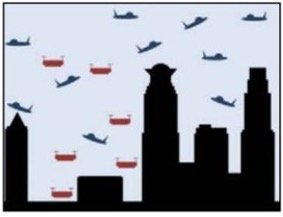
\includegraphics[width=\textwidth]{img/full-mix.jpg}
        \caption{Full-Mix}
        \label{full-mix}
    \end{subfigure}
    \begin{subfigure}{.23\textwidth}
        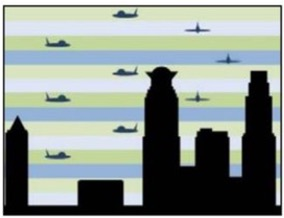
\includegraphics[width=\textwidth]{img/layers.jpg}
        \caption{Layers}
        \label{layers}
    \end{subfigure}
    \begin{subfigure}{.23\textwidth}
        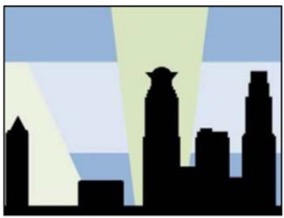
\includegraphics[width=\textwidth]{img/zones.jpg}
        \caption{Zones}
        \label{Zones}
    \end{subfigure}
    \begin{subfigure}{.23\textwidth}
        
\includegraphics[width=\textwidth]{img/tubes.jpg}
        \caption{Tubes}
        \label{tubes}
    \end{subfigure}
    \caption{Metropolis: Airspace concepts \cite{Schuchardt_2023}.}
    \label{airspace-concepts}
\end{figure}

Simulations by Sunil et al. \cite{Sunil_2015} showed that conflict resolution using the \gls{MVP} and A* algorithms yielded better efficiency and fewer conflicts in less-structured airspace (Full Mix and Layers). 
Layers performed best overall, balancing throughput, safety, and flexibility.


% \subsubsection{Metropolis 2 Project: Separation Management Strategies}

Building on these findings, the Metropolis 2 project explored \gls{ATM} concepts for mixed airspace environments, including both open and constrained regions. 
This second phase addressed practical constraints such as tall urban buildings and complex terrain, where vertically layered airspace may be impractical (e.g., in cities like New York).
The project compared three separation management strategies with varying degrees of centralisation (Figure~\ref{atc-concepts}) \cite{Patrinopoulou_2022}:

\begin{itemize}
    \item \textbf{Centralised:} A single central authority handles pre-flight planning and strategic conflict resolution using global knowledge of all flights.
    \item \textbf{Decentralised:} Each \gls{UAV} is responsible for its trajectory and separation, without access to other flight plans.
    \item \textbf{Hybrid:} Combines strategic central planning with tactical in-flight deconfliction by the agents themselves (a mix of both centralised and decentralised concepts).
\end{itemize}

\begin{figure}[!ht]
    \centering
    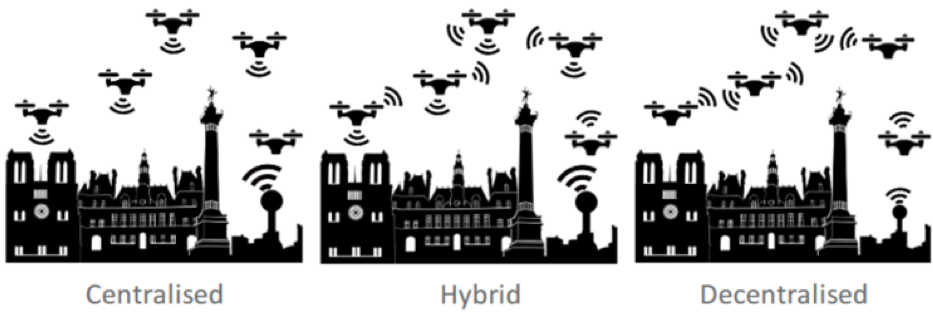
\includegraphics[width=.7\textwidth]{img/metropolis-ii-airspace.png}
    \caption{Metropolis 2: Air traffic control concepts \cite{Badea_2022}.}
    \label{atc-concepts}
\end{figure}

% According to Badea \cite{Badea_2022}, the simulations revealed that each concept has trade-offs. 
% The centralised model achieved the highest route efficiency but lacked scalability. 
% The decentralised model ensured fair access to airspace but struggled with conflict management. 
% The hybrid approach provided the best safety performance and balanced traffic distribution, showcasing the benefits of combining proactive (strategic) and reactive (tactical) elements.

Badea \cite{Badea_2022} found that the centralised model was most efficient but limited in scalability, while the decentralised model promoted fairness but struggled with safety. 
The hybrid model delivered the best balance of safety, flexibility, and scalability, showcasing the benefits of combining proactive (strategic) and reactive (tactical) elements.


% \subsubsection{Implications for the Future of AI in ATM}

% The findings of Metropolis and Metropolis 2 underscore the vital role that \gls{AI} will play in the future of \gls{ATM}. 
% In particular:
% \begin{itemize}
%     \item \Gls{AI} algorithms such as A*, \gls{MVP}, and conflict resolution heuristics are critical for enabling dynamic, decentralised trajectory planning.
%     \item Multi-agent reinforcement learning (MARL) and predictive models could further enhance the hybrid model by learning optimal conflict-avoidance behaviours in real time.
%     \item Strategic \gls{AI} planning systems are needed to anticipate demand surges, optimise vertical and horizontal traffic flow, and ensure robust safety margins under uncertainty.
% \end{itemize}

% The findings from the Metropolis and Metropolis 2 projects highlight the crucial role of \gls{AI} in shaping the future of \gls{ATM}. 
% Key technologies include algorithms like A*, \gls{MVP}, and conflict resolution heuristics for dynamic, decentralised trajectory planning. 
% Additionally, multi-agent reinforcement learning (MARL) and predictive models offer potential for real-time optimisation of conflict-avoidance strategies, while strategic \gls{AI} planning tools are essential for managing traffic flow, anticipating demand peaks, and maintaining safety under uncertainty.

Overall, the Metropolis projects underscore the importance of \gls{AI} in future \gls{ATM}. 
Algorithms like A* and \gls{MVP} support decentralised planning, while multi-agent reinforcement learning (MARL) and predictive models enhance conflict avoidance in real-time. 
Strategic \gls{AI} tools are also vital for managing traffic flow, anticipating demand surges, and maintaining safety in uncertain environments.

% In summary, the future separation management system in high-density urban airspace will likely adopt a hybrid approach powered by \gls{AI}. 
% Such a system would combine centralised strategic optimisation with decentralised, \gls{AI}-driven tactical deconfliction, ensuring both safety and equitable access while adapting to uncertainties in environment, demand, and infrastructure.

